% This is samplepaper.tex, a sample chapter demonstrating the
% LLNCS macro package for Springer Computer Science proceedings;
% Version 2.20 of 2017/10/04
%
\documentclass[runningheads]{llncs}
%
\usepackage{graphicx}
% Used for displaying a sample figure. If possible, figure files should
% be included in EPS format.
%
% If you use the hyperref package, please uncomment the following line
% to display URLs in blue roman font according to Springer's eBook style:
% \renewcommand\UrlFont{\color{blue}\rmfamily}

\usepackage{booktabs}
\usepackage{subfig}
\usepackage{svg}

\begin{document}
%
\title{Using Nature Inspired Algorithms for Feature Selection in Transaction Fraud Detection}
%
\titlerunning{Using NIA for Feature Selection in Transaction Fraud Detection}
% If the paper title is too long for the running head, you can set
% an abbreviated paper title here
%
\author{Peter Mačinec \and Timotej Zaťko}
%
\authorrunning{Peter Mačinec, Timotej Zaťko}
% First names are abbreviated in the running head.
% If there are more than two authors, 'et al.' is used.
%
\institute{Faculty of Informatics and Information Technologies,\\Slovak University of Technology, Bratislava}
%
\maketitle              % typeset the header of the contribution
%
\begin{abstract}
Credit card payments are still more and more preferred because of convenience. People are using credit cards to pay not only at stores but also in e-shops. However, with the rise of credit card usage, a suitable environment for fraud in transactions arises. The data of transactions are usually collected by the banks, which indicates the usage of data-mining approaches to prevent frauds. The performance of the model is based on several sub-steps and decisions, like data analysis, preprocessing, feature selection, and hyperparameter optimization. In the area of transaction fraud detection, datasets usually contain a lot of features (several hundred) that are however mostly anonymized. Thus we decided to focus on improving model mainly by selecting appropriate features using nature-inspired algorithms. Nature-inspired algorithms proved to be powerful methods in such optimization tasks. Experiments showed that a proper combination of machine learning model with feature selection using nature-inspired algorithms has the potential to help to prevent transaction frauds. Out of 5 nature-inspired algorithms, the Grey Wolf Optimizer achieved the best results. It improved the model by 1.4\% (ROC AUC) while selecting half of the features in comparison with a recursive feature elimination.

\keywords{transaction fraud detection \and machine learning classification \and nature inspired algorithms \and feature selection \and bat algorithm.}
\end{abstract}
%
%
%
\section{Introduction}

Payments with credit cards are nowadays still more preferred over using cash. Using a credit card is not only more comfortable for people, but even also more safe than carrying cash in wallet when it comes to a higher amount of money. However, the number of transaction frauds is arising alongside with usage of credit cards. The number of transactions and the ability to obtain data from them indicates the need for automatic detection of suspicious payments.

Data of performed transactions via credit cards are naturally collected by companies and banks to produce statistics or investigate frauds. Therefore, transaction fraud detection can be interpreted as a data mining problem, concretely binary classification. The majority of existing datasets of transaction frauds contain a lot of features, however, most of them are usually anonymized. Thus, the model will rely also on proper feature selection. In such cases, where feature selection is a very important part of the problem, powerful metaheuristic search methods like nature-inspired algorithms can be used.

In this paper, we propose a novel method for detection frauds in transactions using aspects of data analysis, machine learning, and nature-inspired algorithms. The basis of our method lies in the training machine learning model on the best features selected by the nature-inspired algorithm. More nature-inspired algorithms are compared to choose the best one for this problem.


\section{Related works}

The number of transaction frauds is arising alongside with usage of credit cards. To help prevent transaction frauds, common data-mining techniques are available. However, data are in most cases very specific and there is no method suitable to all problems. Addressing that, a comparative study of various machine learning techniques, mostly neural networks, for credit card fraud detection was performed~\cite{Sadgali2019}. Common algorithms like Support Vector Machines~\cite{Wiese2009} or Random Forest~\cite{Xuan2018} were also examined. Another and very specific way to detect frauds is by using Genetic programming~\cite{Assis2013}. Genetic programming has proven to be very effective for this problem, achieving significant improvements (up to almost 17\% compared to corporation baseline).

Each transaction can be viewed separately as one unit, but also whole transaction history can be considered. To create a model that is resistant to changes in transactions, modeling time series using Long-Short Term Memory (LSTM) recurrent neural networks seems to be the right way~\cite{Wiese2009}.

Publicly available datasets for transaction fraud detection usually contain a lot of features. It is necessary to put special effort into the feature selection phase in such cases. Nature-inspired algorithms proved to be very powerful for feature selection problems in previous research. When using metaheuristic approaches like nature-inspired algorithms, feature selection problem can be interpreted as combinatorial optimization problem~\cite{Wang2016}.

Rough sets are popular when using nature-inspired algorithms for feature selection (more about rough sets theory used in data mining in~\cite{Slimani2013}). Rough sets were used in combination with Firefly Algorithm~\cite{Banati2011}, Particle Swarm Optimization~\cite{Wang2007}, or Bat Algorithm~\cite{Emary2014}. The majority of works used multiple datasets for their experiments to prove nature-inspired algorithms power.

There are also other surveys focused mainly on the usage of nature-inspired algorithms for feature selection~\cite{Kauser2018,Wang2016,Yang2020}. Further algorithms were researched, like Artificial Bees Colony, Cuckoo Search, Ant Colony Optimization, or Genetic Algorithms.

%  opis použitého algoritmu - aj s odôvodnením výberu algoritmu
%  opis vykonaných experimentov - opis použitého datasetu, opis cieľu a postupu
% experimentu, opis nastavení algoritmu (odôvodnenie prečo zvolené
% nastavenia), opis metrík, ktorými experiment vyhodnocujete... ak sa
% porovnávate s existujúcimi riešeniami, nezabudnite ich citovať, prípadne aj
% stručne opísať
%  Vyhodnotenie / Evaluation - prehľadné výsledky experimentov (formou
% textového opisu, grafov, tabuliek, ...)
%  Záver / Conclusion
%  Použitá literatúra / References - používajte LNCS štýl odkazovania sa na
% zdroje, pokyny nájdete aj v šablóne (príklady tu alebo tu, štýl pre správcu
% citácii Mendeley)


\section{Problem definition}


% TODO: opisat nas problem
% TODO: spomenut - nevyvazene triedy, velmi vela features, chyba domenovat znalost (features) kvoli anonymizacii
% TODO: opisat dataset - nejaky grafy, pocty pozorovani, features

The majority of datasets available for data science research of transaction fraud detection have the same characteristics - highly imbalanced data, a lot of features, and the majority of features are anonymized.

Our method will be trained and evaluated on a dataset from Kaggle competition EEE-CIS Fraud Detection\footnote{https://www.kaggle.com/c/ieee-fraud-detection/data}. As usual in problems of transaction fraud detection, a lot of features of different types are available - 434 features describing demography, credit card, the transaction itself, etc. The majority of features are anonymized or the meaning of them is not clear. In this case, we must be careful to avoid labels leak from some features and also in interpreting data analysis or models result when talking about anonymized features. This dataset contains almost 600k samples, that is appropriate for machine learning algorithms. However, data are highly imbalanced - class distribution can be seen in figure~\ref{fig:classes}. When training and evaluating models, one should be careful when data are imbalanced.

We cannot handpick the features, because the data are anonymized so we lack the domain knowledge. Hence we need to apply some methods for feature selection. Also, manually hand-picking for that large amount of features would be nearly impossible. Another motivation for feature selection is that it reduces model complexity and improves its interpretability.

\begin{figure}[ht]
	\begin{center}
	    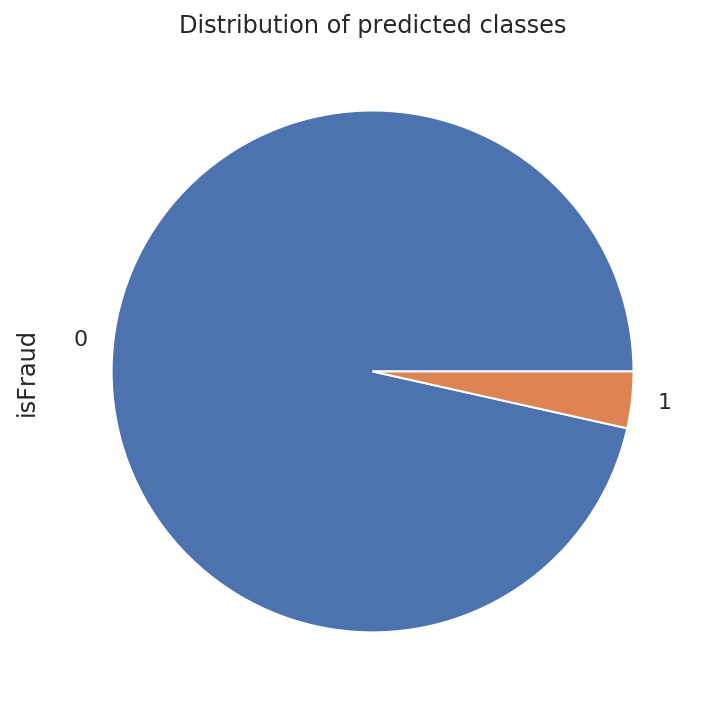
\includegraphics[width=0.5\textwidth]{figures/class_distribution.png}
    \end{center}
	\caption{Predicted classes distribution - data are highly imbalanced.}
	\label{fig:classes}
\end{figure}


\section{Method proposal}

% TODO: Len kratko, co navrhujeme - feature selection na nejaky model pomocou nejakeho prirodou inspirovaneho algoritmu.

% usage of nature inspired algorithm proved to optimize feature selection much better than baseline well-known methods and overperforms  using power of nature inspired algorithms to address the problem of a lot of anonymized features available in existing datasets. Combination of machine learning and nature inspired algorithms proved to be the wa

% Proper data analysis in combination with training machine learning models can help to prevent frauds. Problem of choosing correct features without knowing their meaning with goal to improve detection performance can be seen as optimization problem. Nature inspired algorithms are known to be very powerful for optimization problems.

% 440 features at the end

To improve a machine learning models for the transaction fraud detection in a way of interpretability and complexity, we propose to use nature-inspired algorithms for feature selection. We will try several nature-inspired algorithms and compare them to find out which one is most suitable for our problem. We decided to use the following algorithms: Firefly Algorithm (FA) \cite{fister2013comprehensive}, Cuckoo Search (CS) \cite{yang2009cuckoo}, Bat Algorithm (BA) \cite{yang2010new}, Flower Pollination Algorithm (FPA) \cite{yang2012flower}, Grey Wolf Optimizer (GWO) \cite{Mirjalili_Mirjalili_Lewis_2014} since they were already used for feature selection in related works or they performed extraordinarily in other types of tasks.

These algorithms will be trying to find the optimal set of features, which will be represented as a binary vector. The size of this vector will be equal to the number of features. Ones in the vector will indicate that the respective features are selected and nulls vice-versa. The nature-inspired algorithms won't be directly optimizing that binary vector, they will be optimizing vector of floats with values in $<0, 1>$ which will be later transformed to binary vector (Figure \ref{fig:projection}). The model will be fitted with the selected features from the solution vector.

\begin{figure}[ht]
	\begin{center}
	    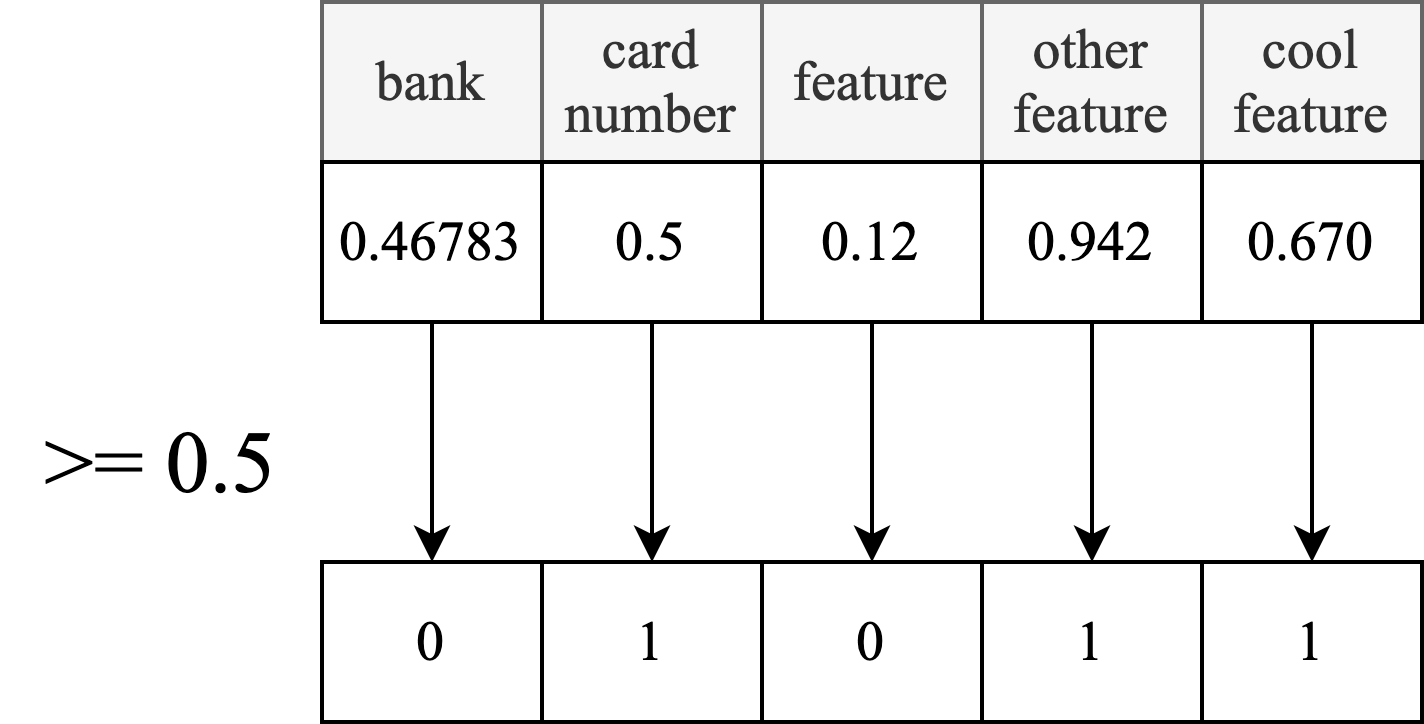
\includegraphics[width=8cm]{figures/projection.png}
    \end{center}
	\caption{Projection from the vector of floats which is being optimized by nature-inspired algorithms to the binary vector representing wether feature is selected or not.}
	\label{fig:projection}
\end{figure}

To prevent overfitting we will do cross-validation ($k=5$) for each solution, the mean score from every one of $k$ fits will represent the fitness of the solution.

% TODO: Mention which were previosly used for feature selection


% TODO: Odôvodnenie výberu optimalizačného algoritmu
% TODO: Detailnejsia analýza hlavného algoritmu
% TODO: Návrh spôsobu nastavenia parametrov
% TODO: Návrh overenia

\section{Preparation}

Before performing experiments, we preprocessed the data. At first, useless columns like id of transaction or those with too many missing values (more than 50\%) are dropped. Our preprocessing pipeline can be devided into two branches - preprocessing of numeric and categorical attributes. In numerical attributes, missing values are filled in with mean value, then all values are normalized (some machine learning algorithms are sensitive to different scales). For categorical attributes, transformation of emails to email domains has been performed, missing values have been filled with most frequent values, small categories (smaller than 5\%) merged into one \textit{other} category and at the end, all features have been one-hot encoded. Also, missing values indicators have been added to both, numerical and categorical attributes.


% TODO: spomenut preprocessing, co sme robili a co z toho vzislo
% TODO: spomenut transformery, one hot, a filter
% TODO: kolko bol finalny pocet features
% TODO: len kratko spomenut ze preco sme sa rozhodli pouzit aky model - decision tree
% TODO: model selection phase

\section{Experiments}

We did several experiemnts in which we compared the following algorithms and their parameters:

\begin{itemize}
	\item Firefly Algorithm ($\alpha = 1$, $\beta_{min} = 1$, $\gamma = 2$)
	\item Cuckoo Search ($p_a = 0.2$, $\alpha = 0.5$)
	\item Bat Algorithm ($A = 0.5$, $r = 0.5$, $Q_{min} = 0.0$, $Q_{max} = 2.0$)
	\item Flower Pollination Algorithm ($p = 0.35$, $\beta = 1.5$)
	\item Grey Wolf Optimizer
\end{itemize}

We will use the algorithm default parameters as they are implemented in \textit{NiaPy} \cite{NiaPyJOSS2018} library based on the original papers. As a baseline models we have chosen the model with all features and model with selected features from \textit{recursive feature elimination with cross-validation}.

\subsection{Experiments strategy}

We chose a \textit{decision tree classifier} as a model on which we will try to find the optimal features. Based on our experiments it achieved the best results considering also the training speed. We kept the default hyper-parameters for this classifier set by scikit-learn library.

Since the dataset is pretty large, we firstly \textit{undersampled} it to achieve the equal size of both classes. Then we shrunk it again to 5\% of its size, so we would be able to make as many experiments as possible (since we did not have enough computing power). We did a train/test split of 80/20.

For each algorithm, we tried several population sizes (10, 20, and 50), for which we did 5 runs of each algorithm. We trained exactly 50 generations. For both, recursive feature elimination and feature selection using nature-inspired algorithms we did 5 fold cross-validation.

\subsection{Results}

When comparing the population sizes, all of the algorithms achieved the best results when the population size was highest (50). The only exception is Cuckoo Search, which found the most optimal solution with population size of 10, however the difference negligible. Table \ref{tab:nia_comparison}. shows the algorithm scores for each population. Figure \ref{fig:nia_train_score_by_algorithm_1}. \& \ref{fig:nia_train_score_by_algorithm_2}.shows the differences in scores between population size of 10 and 50.

% \begin{figure}
%     \centering
%     \subfloat{{ 
%         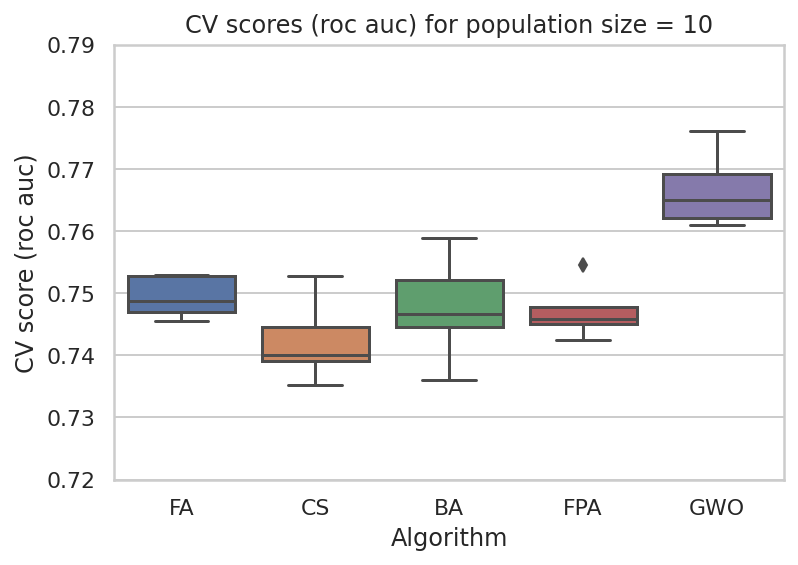
\includegraphics[width=5.5cm]{figures/nia_train_score_by_algorithm_10}
%     }}
%     \qquad
%     \subfloat{{
%         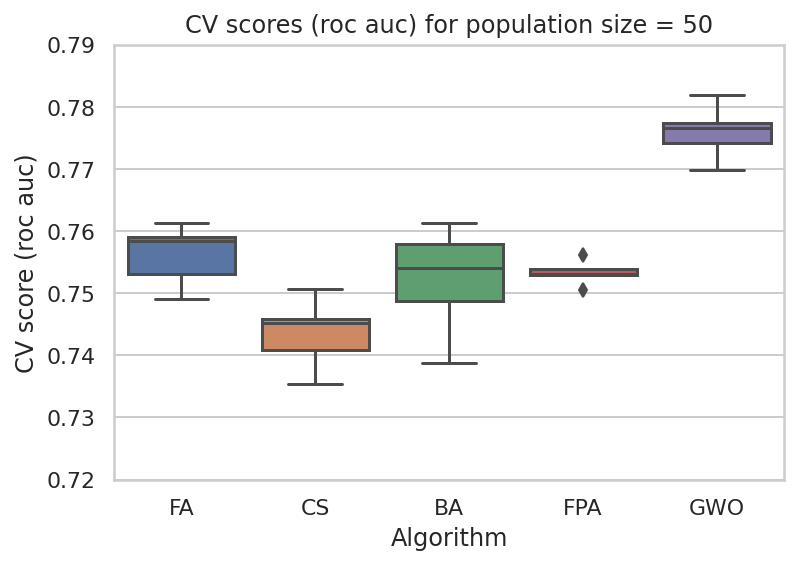
\includegraphics[width=5.5cm]{figures/nia_train_score_by_algorithm_50}
%     }}
%     \caption{Scores of the algorithms by the population size. The scores are slightly higher for population size of 50.}
%     \label{fig:nia_train_score_by_algorithm}
% \end{figure}

\begin{figure}
    \centering
    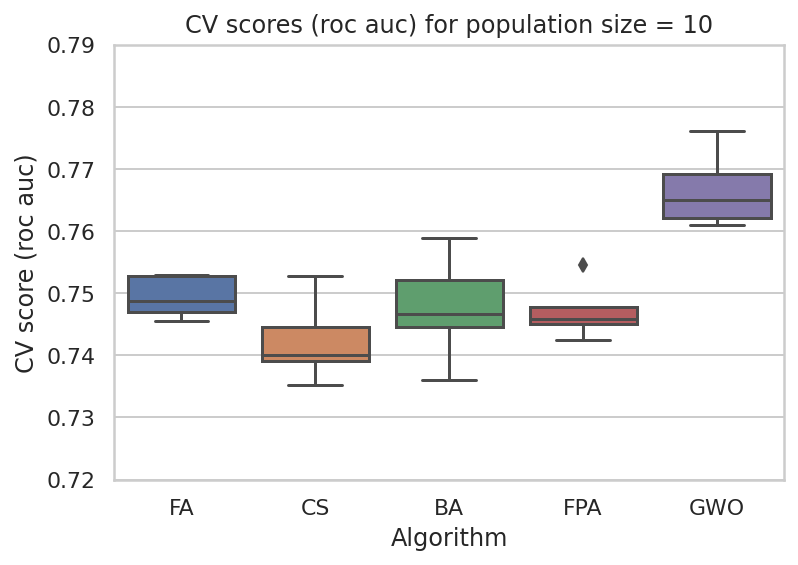
\includegraphics[width=11cm]{figures/nia_train_score_by_algorithm_10}
    \caption{Scores of the nature-inspired algorithms for population size of 10.}
    \label{fig:nia_train_score_by_algorithm_1}
\end{figure}

\begin{figure}
    \centering
    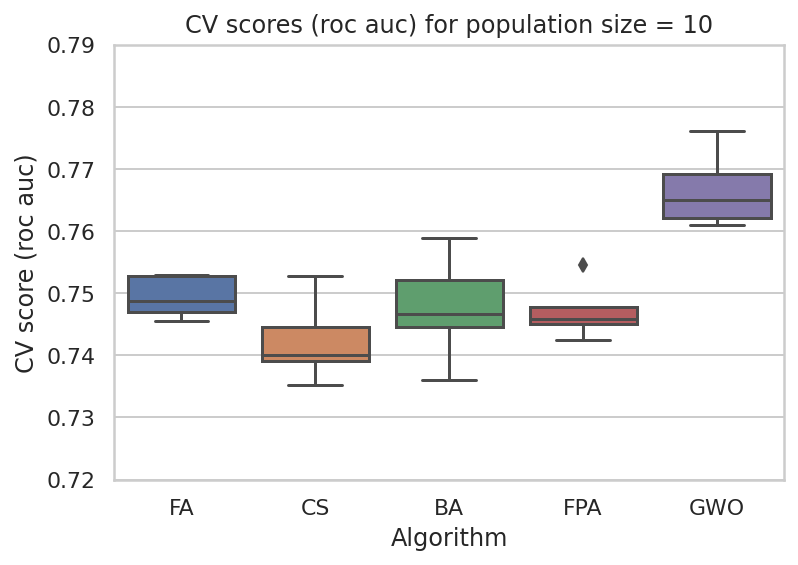
\includegraphics[width=11cm]{figures/nia_train_score_by_algorithm_10}
    \caption{Scores of the nature-inspired algorithms for population size of 50.}
    \label{fig:nia_train_score_by_algorithm_2}
\end{figure}

\def\arraystretch{1.5}
\begin{table}
	\begin{center}
		\caption{Highest train scores (ROC AUC) of nature inspired algorithms by population size. We may notice that Grey Wolf Algorithm (GWO) outperformed all of the other algorithms.} \label{tab:nia_comparison}
	\end{center}
	\begin{center}
		\begin{tabular}{|l|r|r|r|r|r|}
			\hline
			\textbf{Population size \textbackslash Score} & \multicolumn{1}{r|}{\textbf{FA}} & \multicolumn{1}{r|}{\textbf{CS}} & \multicolumn{1}{r|}{\textbf{BA}} & \multicolumn{1}{r|}{\textbf{FPA}} & \multicolumn{1}{r|}{\textbf{GWO}} \\ \hline
			\textbf{10}                                             & 0.753                           & \textbf{0.752}                           & 0.759                           & 0.754                            & 0.776                             \\
			\textbf{20}                                             & 0.757                           & 0.746                           & 0.755                           & 0.750                            & 0.771                             \\
			\textbf{50}                                             & \textbf{0.761}                           & 0.751                           & \textbf{0.761}                           & \textbf{0.756}                            & \textbf{0.782}                             \\ \hline
		\end{tabular}
	\end{center}
\end{table}

All of the nature-inspired algorithms perform roughly the same, except the Grey Wolf Optimizer which outperformed the others (Figure \ref{fig:nia_train_score_by_algorithm}). These differences in results between GWO and other algorithms are significant (there is a sigificant difference in means, t-test; $p-value=0.012$). Looking for the explanation, we found out that only Grey Wolf Algorithm and Bat Algorithm converged during the optimization run. Figure \ref{fig:nia_scores_by_run_1}. \& \ref{fig:nia_scores_by_run_2}. shows the optimization progress of the Firefly Algorithm and Grey Wolf Optimizer, Firefly Algorithm did not converge. If we fine-tuned the parameters of other algorithms, they might converge as well. The fact that GWO does not have any parameters (except the population size) might be an advantage for it in our experiments.

% https://towardsdatascience.com/hypothesis-testing-in-machine-learning-using-python-a0dc89e169ce

\begin{figure}[htp]
	\centering
	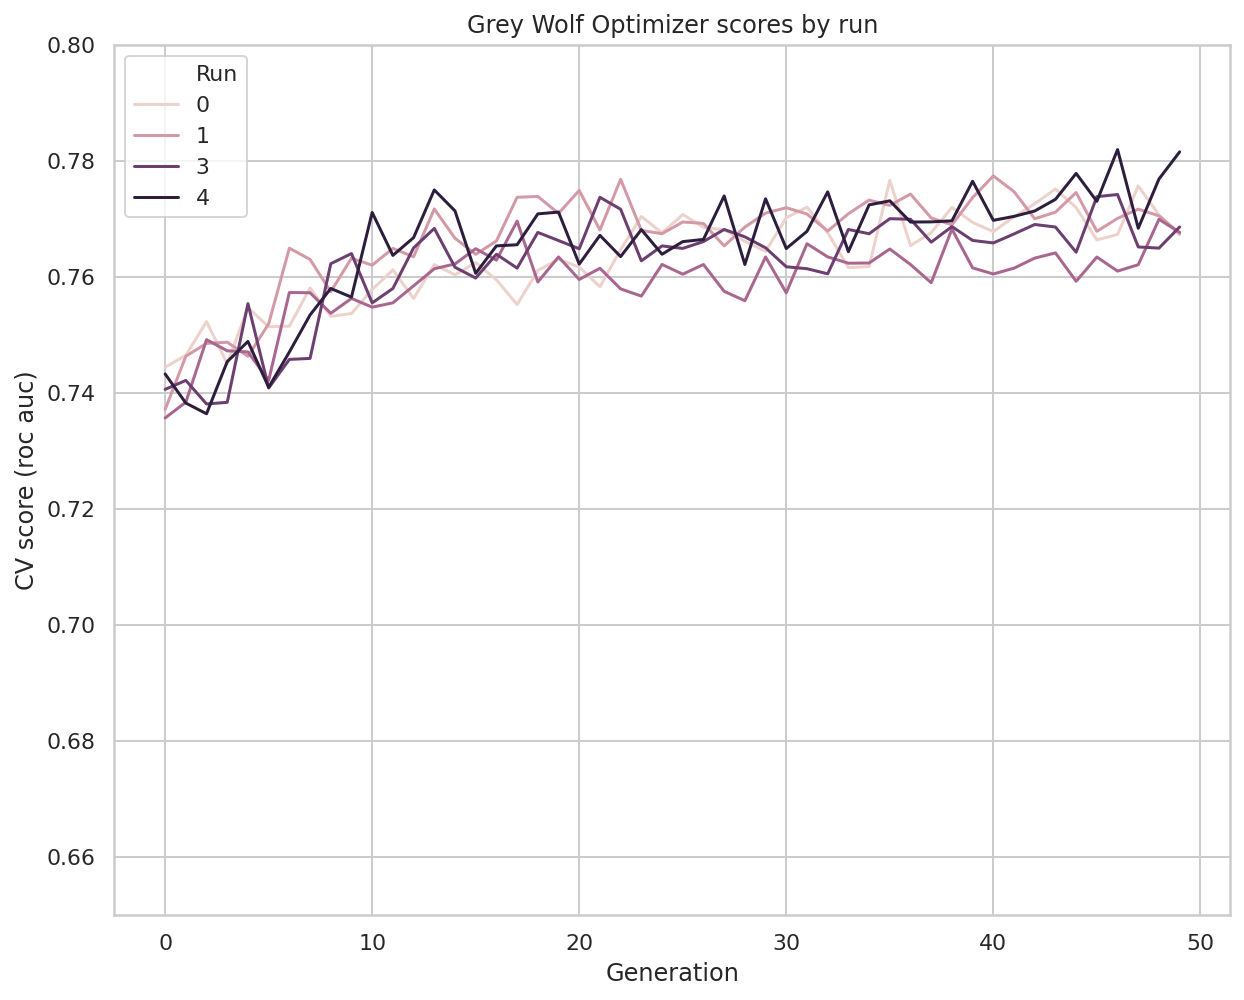
\includegraphics[clip, width=10.5cm]{figures/gwo_scores_by_run}
    \caption{Optimization progress for 5 runs of Grey Wolf Optimizer.}
    \label{fig:nia_scores_by_run_1}
\end{figure}

\begin{figure}[htp]
	\centering
	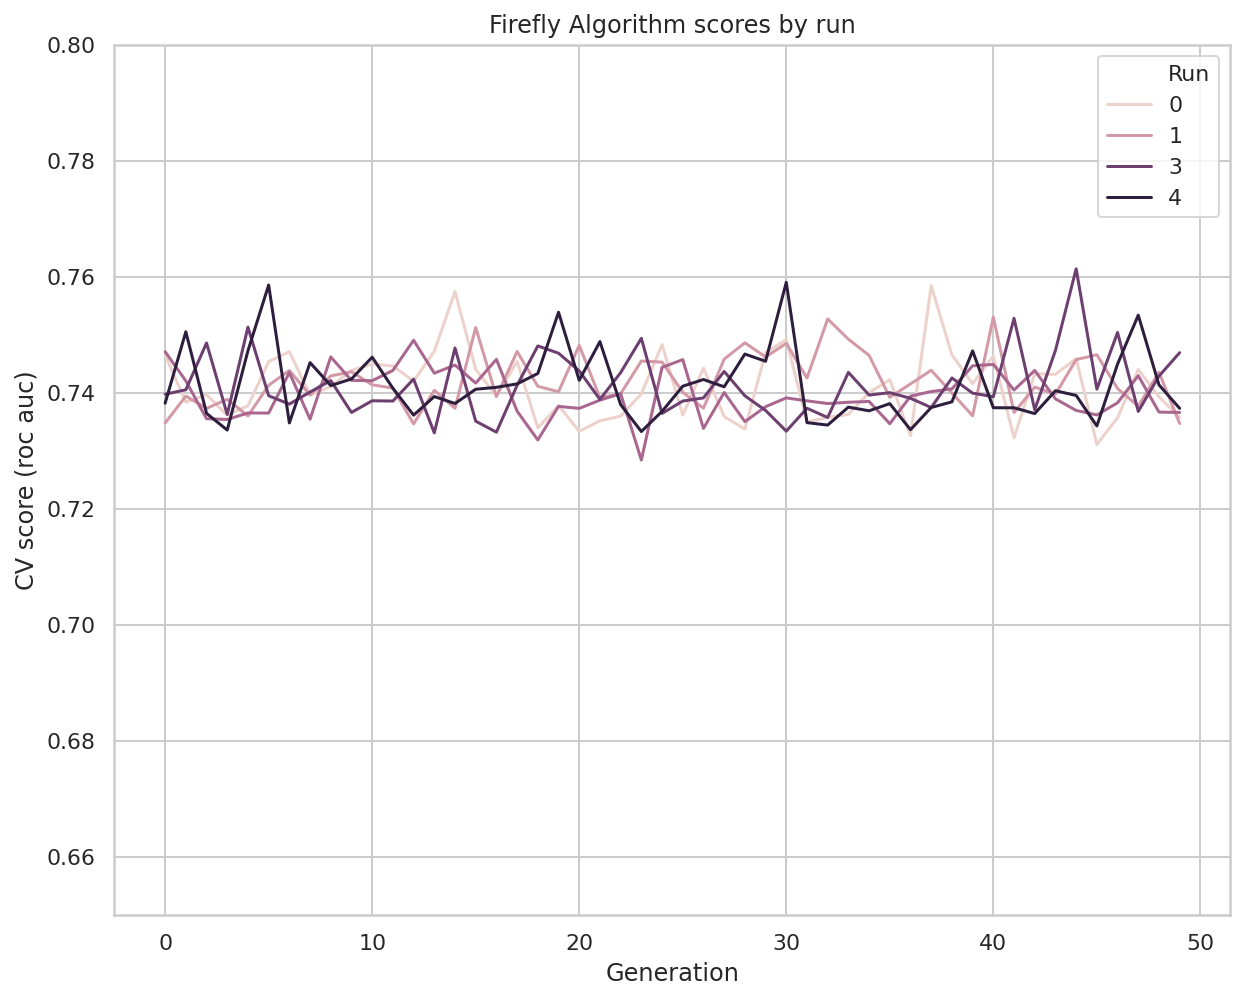
\includegraphics[clip, width=10.5cm]{figures/fa_scores_by_run}
    \caption{Optimization progress for 5 runs of Firefly Algorithm. The optimization process did not converge.}
    \label{fig:nia_scores_by_run_2}
\end{figure}

The best features, selected in the optimization process, were later used to train the final model on test data. These models were compared to the model trained on all features and the model trained on features selected by recursive feature elimination.

The nature-inspired algorithms found a more optimal set of features on the train dataset than recursive feature elimination. However, they achieved worse results on the test dataset. The only exception is Grey Wolf Optimizer, which achieved the best train and test score. The most noticeable difference in the results is the number of selected features by algorithms. All of the algorithms (including recursive feature elimination), selected around $~110$ features, however, GWO selected only 53, this is probably the reason of its results. These results are shown in Table \ref{tab:nia_baseline_comparison}. Figure \ref{fig:nia_selected_features_by_algorithm} shows that GWO selected fewer features in general not only in its best solution.

\begin{table}[]
	\begin{center}
		\caption{Comparison of the baseline models with nature-inspired algorithms. The train score stands for the best score from the optimization. All of the nature-inspired algorithms (except Grey Wolf Optimizer) achieved a better train score than recursive feature elimination, however, they overfit the model which resulted in a worse test scores.} \label{tab:nia_baseline_comparison}
	\end{center}
	\begin{center}
		\begin{tabular}{|l|r|r|r|}
			\hline
			\textbf{Feature selection type} & \textbf{Train score} & \textbf{Test score} & \textbf{Selected features} \\ \hline
			All features                    & N/A                  & 0.713               & 240                                  \\
			Recursive feature elimination   & 0.747                & 0.719               & 112                                  \\
			Firefly Algorithm               & 0.761                & 0.663               & 114                                  \\
			Cuckoo Search                   & 0.753                & 0.718               & 106                                  \\
			Bat Algorithm                   & 0.761                & 0.689               & 125                                  \\
			Flower Pollination Algorithm    & 0.756                & 0.706               & 113                                  \\
			\textbf{Grey Wolf Optimizer}             & \textbf{0.782}                & \textbf{0.733}               & \textbf{53}                                   \\ \hline
		\end{tabular}
	\end{center}
\end{table}

\begin{figure}[ht]
	\begin{center}
	    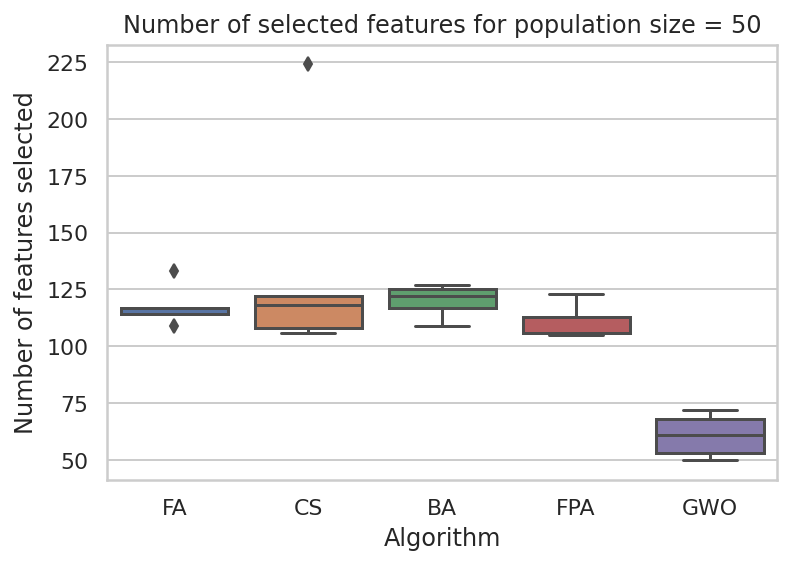
\includegraphics[width=10cm]{figures/nia_selected_features_by_algorithm.png}
    \end{center}
	\caption{Number of selected features by algorithm - Grey Wolf Algorithm selected by far the least number of features.}
	\label{fig:nia_selected_features_by_algorithm}
\end{figure}

\section{Conclusion}

In our experiments, we found out Grey Wolf Optimizer as the best nature-inspired algorithm for feature selection. It achieved significantly better results than other nature-inspired algorithms and better results that recursive feature elimination.

GWO alongside Bat Algorithm was the only nature-inspired algorithms that were able to converge during the optimization process. We assume that other algorithms might converge too if we experimented with their parameter settings. We consider the fact, that GWO does not have any parameters other than population size as a big strength, because it saves a significant amount of optimization time.

In comparison with traditional ways of feature selection (recursive feature elimination), all of the nature-inspired algorithms were able to find better solutions on the training dataset, however, they overfit most of the time. Moreover, the feature selection using nature-inspired algorithms was much slower.

% TODO: concusion in the topic of transaction fraud detection

\bibliographystyle{splncs04}
\bibliography{references}

\end{document}
